\documentclass{./packages/homework}
\usepackage{./packages/caratula}
\usepackage{amssymb}
\usepackage{graphicx}
\usepackage{caption}
\usepackage{subfig}

\graphicspath{./files/src/media/}
\renewcommand{\contentsname}{contenidos}
\renewcommand{\refname}{Referencias}
\renewcommand\qedsymbol{$\blacksquare$}
\renewcommand{\lstlistingname}{Algoritmo}% Listing -> Algorithm
\renewcommand{\figurename}{Figura}% Listing -> Algorithm
\renewcommand\thesubfigure{\roman{subfigure}}
\captionsetup[subfloat]{labelformat=empty}

\lstdefinelanguage{pseudo}{
  morekeywords={
    pre,
    post,
    if,
    while,
    for,
    in,
    out,
    proc,
    inout,
    do,
    and,
    not,
    return,
    break,
    raise
  },
  sensitive=false, % keywords are not case-sensitive
  morecomment=[l]{//}, % l is for line comment
  morecomment=[s]{/*}{*/}, % s is for start and end delimiter
  keywordstyle=\color{black}\textbf,
  commentstyle=\color{gray},
  morestring=[b]", % defines that strings are enclosed in double quotes
  inputencoding=utf8,
  extendedchars=true,
  literate=
    {λ}{$\lambda$}1
    {α}{$\alpha$}1
    {ε}{$\epsilon$}1
    {Λ}{$\Lambda$}1
    {>=}{$\geq$}2
    {<=}{$\leq$}2
}

\newcommand{\TODO}[1]{
  {\noindent \color{red} [#1]}
}

\hyphenation{co-rres-pon-der}
\hyphenation{li-neal}


\begin{document} 

% caratula
\titulo{TP 3: Métodos Iterativos}
\subtitulo{}
\fecha{Noviembre 24, 2022}
\materia{Métodos Numéricos}
\grupo{Grupo 18}

\integrante{Vekselman, Nat\'an}{338/21}{natanvek11@gmail.com}
\integrante{Arienti, Federico}{316/21}{fa.arienti@gmail.com}
\integrante{Manuel Lakowsky}{511/21}{mlakowsky@gmail.com}
\integrante{Brian Kovo}{1218/21}{brian.ilank@gmail.com}

\maketitle


% palabras clave y resumen
\addtocontents{toc}{\protect\setcounter{tocdepth}{0}}
\section*{resumen}
\addtocontents{toc}{\protect\setcounter{tocdepth}{3}}
Los \textit{métodos iterativos} representan una forma alternativa y eficiente para la resolución de sistemas lineales. Dadas las condiciones necesarias, permiten aproximar el resultado de un sistema en tiempo cuadrático, sin amortización. Es decir, logran una complejidad  menor a la que se logra con la mayoría de los otros métodos convencionales ---como lo son aquellos que requieren un paso previo de factorización---, cuyo costo no amortizado suele ser cúbico.

\vspace{1em}
En este trabajo evaluaremos la eficiencia de dos métodos iterativos: el método de \textit{Jacobi} y el método de \textit{Gauss-Seidel}, como alternativas para la resolución del algoritmo de \textit{PageRank} ---desarrollado en el tp1--- sobre una serie de casos de test. Para ello, se propondrá una posible implementación en C++ de ambos métodos y se contrastará su eficiencia con una tercera implementación basada en el método de la \textit{eliminación gaussiana} con \textit{sustitución inversa}.

A su vez, extenderemos éste análisis para evaluar el comportamiento de los tres métodos en función de la \textit{densidad} del grafo de entrada, para distintas familias de redes. 

\vspace{1em}
\noindent Palabras clave: método de Jacobi, Gauss-Seidel, Eliminación Gaussiana, PageRank.


% contenido
% \newpage
\vspace{2em}
\tableofcontents
\newpage

% potencia
\section{Introducción teórica}
% === INTRO === %

\vspace{1em}
\subsection{Métodos iterativos}
Los \textit{métodos iterativos} son procedimientos que nos permiten resolver algunos sistemas de ecuaciones lineales del tipo $\mathbf{A}x = b$. Contrario a los \textit{métodos exactos} ---como la \textit{Eliminación Gaussiana}--- que obtienen su resultado en un número finito de pasos, los métodos iterativos generan una sucesión $\{ x^{(k)} \}_{k \in \mathbb{N}_0}$ que, de converger, lo hace a la solución del sistema.

\vspace{1em}
Como esquema básico, dado un $x^{(0)}$ inicial, se define de manera genérica una sucesión iterativa  $\{ x^{(k)} \}_{k \in \mathbb{N}_0}$ de la siguiente manera:

\begin{equation}\label{sucesion}
    x^{(k+1)} = \mathbf{T}x^{(k)} + c
\end{equation}

\vspace{1em}
\noindent donde $\mathbf{T}$ se denomina \textit{matriz de iteración} y $c$ es un vector. En particular, $x^{(k)}$ va a converger a la solución de un sistema, para cualquier vector $x^{(0)}$ inicial, si y sólo si el radio espectral de la matriz de iteración \textbf{T} es menor a 1. Es decir:

\begin{equation}\label{espectral}
    \rho(\mathbf{T}) = max\{|\lambda|\ :\ \lambda \: \text{\textit{autovalor de} \textbf{T}}\}\ <\ 1
\end{equation}

\vspace{3em}
En este informe, trabajaremos con los métodos de \textit{Jacobi} y \textit{Gauss-Seidel} para la resolución de sistemas $\mathbf{A}x = b$. Estos descomponen a la matriz \textbf{A} de la siguiente forma: 

\begin{equation}
    \mathbf{A} = \mathbf{D} - \mathbf{L} - \mathbf{U}
\end{equation}

\vspace{1em}
\noindent donde $\mathbf{D}$ es la diagonal de $\mathbf{A}$, $\mathbf{L}$ contiene los elementos negados por debajo de la misma y $\mathbf{U}$ los elementos negados por encima. 

\vspace{1em}
\noindent Los esquemas para ambos métodos son los siguientes:

\vspace{1em}
\begin{center}
    \textit{Método de Jacobi}
\end{center}

\begin{equation} \label{jacobi}
    x^{(k+1)} = \textbf{D}^{-1} (\textbf{L} + \textbf{U}) x^{(k)} + \textbf{D}^{-1} b 
\end{equation}

\vspace{2em}
\begin{center}
    \textit{Método de Gauss-Seidel}
\end{center}

\begin{equation}\label{gauss-seidel}
    x^{(k+1)} = (\mathbf{D} - \mathbf{L})^{-1} \mathbf{U} x^{(k)} + (\mathbf{D} - \mathbf{L})^{-1} b
\end{equation}

\vspace{1em}
Se puede demostrar que, de converger, ambos métodos lo harán a la solución del sistema pedido. Requerimos adicionalmente, para su aplicación, que $\mathbf{A}$ sea una matriz sin elementos nulos en la diagonal. De lo contrario, no se podrán calcular las inversas de $\mathbf{D}$ y $\mathbf{D} - \mathbf{L}$.





% === IMPLEMENTACION === %

\vspace{2em}
\subsection{Implementación}

% jacobi
\vspace{2em}
\subsubsection{Método de Jacobi}
Definamos la siguiente aridad para una implementación posible del Método de Jacobi:

\begin{align*}
    \text{\textit{jacobi}}&:\ \text{\textit{matriz}}_{n \times n}\ \mathbf{A}\ \times\ \text{\textit{vector}}_n\ \text{b}\ \times\ \text{\textit{nat} q}\ \times\ \text{\textit{real} t}\
    \longrightarrow\ \text{\textit{vector}}_n\ \text{x}
\end{align*}

\vspace{1em}
\noindent donde $n$ es un natural, \textbf{A} es una matriz con elementos distintos a cero en la diagonal, \textit{q} es un número que indica la cantidad máxima de iteraciones a realizar y \textit{t} $\geq$ 0 representa la tolerancia mínima a partir de la que se considera la convergencia de una solución.

\vspace{1em}
Si la matriz $\mathbf{A} = \mathbf{D} - \mathbf{L} - \mathbf{U}$, satisface que $\rho(\mathbf{D}^{-1}(\mathbf{L} + \mathbf{U})) < 1$, entonces el método de Jacobi convergerá a una solución del sistema $\mathbf{A}x = b$. Proponemos el siguiente algoritmo:

\vspace{1em}
\lstinputlisting[mathescape=true, escapechar=@, language=pseudo, label=algo_jacobi, caption={Pseudocódigo para el \textit{Método de Jacobi}.}]{files/src/.code/jacobi.pseudo}

\vspace{1em}
Notamos que la complejidad del algoritmo es del orden de $\Theta(q * n^2)$ en el peor caso. En consecuencia, se debe precisar con cuidado la cantidad de iteraciones a realizar para que el factor $q$ sea despreciable. Del mismo modo, una selección de $t$ correcta, acorde al uso, puede resultar en mejoras considerables en la complejidad promedio. % Como se precisará más adelante, notamos en nuestra experimentación que para $n \leq 3000$ bastó de manera holgada $q = 100$ para lograr un error absoluto $L_1$ menor a $10^{-5}$.


    

% gauss seidel
\vspace{2em} 
\subsubsection{Método de Gauss-Seidel}
De manera similar, definimos la siguiente función que implementa el Método de Gauss-Seidel:

\begin{align*}
    \text{\textit{gauss\_seidel}}&:\ \text{\textit{matriz}}_{n \times n}\ \mathbf{A}\ \times\ \text{\textit{vector}}_n\ \text{b}\ \times\ \text{\textit{nat} q}\ \times\ \text{\textit{real} t}\
    \longrightarrow\ \text{\textit{vector}}_n\ \text{x}
\end{align*}

\vspace{1em}
\noindent donde, nuevamente, $n$ es un natural, \textbf{A} es una matriz con elementos distintos a cero en la diagonal, \textit{q} es un número que indica la cantidad máxima de iteraciones a realizar y $t \geq 0$  representa la tolerancia mínima a partir de la que se considera la convergencia de una solución.

\vspace{1em}
Si la matriz $\mathbf{A} = \mathbf{D} - \mathbf{L} - \mathbf{U}$, satisface que $\rho((\mathbf{D} - \mathbf{L})^{-1}(\mathbf{U})) < 1$, entonces el método de Gauss-Seidel convergerá a una solución del sistema $\mathbf{A}x = b$. Proponemos el siguiente algoritmo, similar al anterior:

\vspace{1em}
\lstinputlisting[mathescape=true, escapechar=@, language=pseudo, label=algo_jacobi, caption={Pseudocódigo para el \textit{Método de Gauss-Seidel}.}]{files/src/.code/gauss_seidel.pseudo}

\vspace{1em}
\noindent Nuevamente, su complejidad temporal es $\Theta(q * n^2)$ en el peor caso.

\vspace{1em}
Observamos que ambos algoritmos aplican ciertas heurísticas que pueden ayudar a reducir su complejidad temporal. Por un lado, se utiliza un vector inicial aleatorio con norma $L_2 = 1$. Esto nos permite evitar aquellas entradas que causan un comportamiento de peor caso de manera determinística, a cuestas que una ejecución particular del algoritmo pueda resultar menos eficiente de manera aleatoria. Por el otro lado, se considera la norma $L_2$ entre dos soluciones consecutivas, como medida de similitud, para definir un quiebre temprano en la iteración externa de los algoritmos en función del parámetro $t$. 




% gauss elim
\vspace{2em}
\subsubsection{Eliminación Gaussiana y representación de matrices}

Por último, para poder realizar una comparación entre los \textit{métodos iterativos} y los \textit{métodos exactos}, propondremos una representación de matriz adecuada y un algoritmo eficiente de \textit{eliminación gaussiana} con \textit{sustitución inversa} para la resolución de \textit{PageRank}.

\vspace{1em}
Dadas las cualidades ralas de las matrices asociadas al problema, decidimos trabajar con la siguiente representación: un vector de vectores \textit{sparse} de la biblioteca \textit{Eigen}, que se implementa sobre un esquema CRS ---\textit{compressed row storage}--- para el indexado a memoria. En el apartado (\ref{representacion}.) explicamos en más detalle esta decisión.

\vspace{1em}
En tanto su implementación, proponemos los siguientes algoritmos para \textit{eliminación gaussiana} y \textit{sustitución inversa}, que aprovechan las herramientas que brinda \textit{Eigen}:

\vspace{1em}
\lstinputlisting[mathescape=true, language=pseudo, label=e, caption={Pseudocódigo para la \textit{Eliminación Gaussiana}.}]{files/src/.code/eg2.pseudo}

\vspace{1em}
\noindent donde \textit{filas}(\textbf{A}) refiere a una función que retorna la cantidad de filas en la matriz \textbf{A}, \textit{v.coeff(i)} refiere a un acceso al $i$-ésimo elemento del vector $v$ y \textit{v.pruned($\alpha$, $\varepsilon$)} es una función que reemplaza los elementos explícitos en la memoria del vector $v$ con valor absoluto menor a $\alpha \cdot \varepsilon$ con un cero implícito.

\vspace{1em}
Notamos que la utilización de la función \textit{pruned} permite mantener una matriz esparsa a lo largo del proceso de eliminación a cuestas de una pérdida de precisión en los resultados. Por ello, una buena selección de $\varepsilon$ es fundamental para el buen funcionamiento del algoritmo. Su interpretación es la siguiente: la tolerancia $\varepsilon$ denota el mínimo valor a considerar no nulo durante el proceso de eliminación.

\vspace{1em}
\noindent %Para la \textit{sustitución inversa}, por su parte, proponemos el siguiente código:

\vspace{1em}
\lstinputlisting[mathescape=true, language=pseudo, label=sinv, caption={Pseudocódigo para \textit{Sustitución Inversa}.}]{files/src/.code/sinv.pseudo}

\vspace{1em}
El algoritmo (\ref{sinv}.), por su parte, utiliza las funciones \textit{iterador(v)}, que retorna un iterador sobre los elementos no nulos del vector $v$, y \textit{pos(it)}, que retorna la posición ---contando ceros--- a la que está apuntando el iterador $it$. 




\vspace{2em}
\subsubsection{¿Por qué usamos \textit{vector$<$SparseVector$>$} como representación?}\label{representacion}

\vspace{1em}
Nuestra primera implementación `naive' de la \textit{Eliminación Gaussiana} con Eigen se puede apreciar en el Algoritmo (\ref{g1}.).

\vspace{1em}
A pesar de ser un código sencillo, creíamos que al usar las funciones de la biblioteca y la representación \textit{SparseMatrix} podríamos obtener una ventaja en velocidad. Pero la hipótesis fue claramente refutada con los tiempos que obtuvimos: el test \textit{15\_segundos}, por su cuenta, demoró tres minutos y trece segundos en ejecutar en una de nuestras máquinas.

\vspace{1em}
Observamos que la asignación de la línea 13 es una operación muy ineficiente. Esto tiene bastante sentido, ya que \textit{SparseMatrix} está implementada usando \textit{CRS} y por ende todos los elementos se encuentran contiguos en un único vector. Insertar y editar un índice en el medio de éste es un proceso costoso.
 
\vspace{1em}
Concluimos de la observación anterior que, en caso de tener un \textit{vector$<$SparseVector$>$} ---donde podamos hacer reemplazos de una fila por otra considerablemente rápido---, además de seguir aprovechando las operaciones optimizadas que provee \textit{Eigen}, podríamos acelerar considerablemente el algoritmo. Teniendo esto en mente, probamos la implementación detallada en el apartado anterior.

\vspace{1em}
\lstinputlisting[mathescape=true, language=pseudo, label=g1, caption={Código C++ de la primera implementación de \textit{Eliminación Gaussiana}.}]{files/src/.code/eg1.pseudo}

\vspace{1em}
Esta estrategia resultó considerablemente mejor, ya que ---en nuestras máquinas--- resuelve correctamente el test \textit{15\_segundos} en aproximadamente 2.5 segundos y el test \textit{30\_segundos} en 5, dado\footnote{Un comentario necesario es que los tiempos mencionados dependen de $\varepsilon$. Esto es relevante ya que modificar esta variable cambia considerablemente la velocidad del algoritmo. Por ejemplo, con $\varepsilon = 10^{-4}$ el algoritmo termina ambos tests en menos de un segundo, pero con $\varepsilon = 10^{-6}$, demora 6 segundos en el de 15 y 11 en el de 30. No profundizaremos en cómo varía la velocidad respecto a $\varepsilon$.
} $\varepsilon = 10^{-5}$.

% \vspace{1em}
% Otra optimización que consideramos fue implementar la resta realizada en la línea 9 del algoritmo. Usando los iteradores de Eigen y un vector auxiliar como se muestra en la siguiente figura.

% \vspace{1em}
% \lstinputlisting[mathescape=true, language=pseudo, label=e, caption={Pseudocódigo de la segunda implementación de la Eliminación Gaussiana}]{files/src/.code/eg3.pseudo}

% \vspace{1em}
% Esta implementación es un poco más rápida ya que corre el test de 15 en 2 segundos y el de 30 en 4, pero no nos parecio una diferencia tal que justifique la pérdida de claridad en el código, por lo que decidimos dejar la implementación anterior.

%\vspace{1em}
%Cabe destacar que para el \textit{tp1} realizamos una implementación similar, usando un vector de vectores de \textit{pair} como representación. Sin embargo, esta resultó más lenta que la versión final usando \textit{Eigen}, probablemente se deba al manejo de memoria y la velocidad de los iteradores de la biblioteca.

\newpage

%\section{¿Por qué usamos $vector<SparseVector>$ como representación?}
%Nuestra primer implementación "naive" de la eliminación gaussiana usando Eigen fue la siguiente:

\vspace{1em}
\lstinputlisting[mathescape=true, language=pseudo, label=e, caption={Pseudocódigo de la primer implementación de la Eliminación Gaussiana}]{files/src/.code/eg1.pseudo}

\vspace{1em}
A pesar de ser un código sencillo, creíamos que al usar las funciones de Eigen podríamos obtener ventaja en velocidad pero la hipótesis fue claramente refutada por los 3 minutos 13 segundos que demoró en terminar el test de 15 segundos.

\vspace{1em}
Observamos que la asignación de la línea 9 era una operación muy ineficiente. Esto tiene bastante sentido ya que SparseMatrix esta implementada usando CSR y por ende todos los elementos se encuentran contiguos en un único vector, entonces insertar y editar en el medio de este es un proceso costoso.
 
\vspace{1em}
Concluimos de la observación anterior que en caso de tener un $vector<SparseVector>$, donde podamos hacer reemplazos de una fila por otra considerablemente rápido, además de seguir aprovechando las operaciones optimizadas de Eigen, sería una buena opción. Teniendo esto en mente, probamos la siguiente implementación:

\vspace{1em}
\lstinputlisting[mathescape=true, language=pseudo, label=e, caption={Pseudocódigo de la segunda implementación de la Eliminación Gaussiana}]{files/src/.code/eg2.pseudo}

\vspace{1em}
Definitivamente esta estrategia es superior ya que resuelve correctamente el test de 15 segundos en aproximadamente 2.5 segundos y el de 30 en 5.

% \vspace{1em}
% Otra optimización que consideramos fue implementar la resta realizada en la línea 9 del algoritmo. Usando los iteradores de Eigen y un vector auxiliar como se muestra en la siguiente figura.

% \vspace{1em}
% \lstinputlisting[mathescape=true, language=pseudo, label=e, caption={Pseudocódigo de la segunda implementación de la Eliminación Gaussiana}]{files/src/.code/eg3.pseudo}

% \vspace{1em}
% Esta implementación es un poco más rápida ya que corre el test de 15 en 2 segundos y el de 30 en 4, pero no nos parecio una diferencia tal que justifique la pérdida de claridad en el código, por lo que decidimos dejar la implementación anterior.

\vspace{1em}
Cabe destacar que para el tp1 hicimos una implementación muy similar, a la presentada, usando $vector<pair>$ como representación pero era bastante mas lenta que la versión final usando Eigen, probablemente se deba al manejo de memoria y la velocidad de los iteradores de la librería mencionada.

\vspace{1em}
Un comentario necesario es que los tiempos mencionados fueron calculados usando $Epsilon = 10^{-5}$. Esto es relevante ya que modificar esta variable cambia considerablemente la velocidad del algoritmo. Por ejemplo con $Epsilon = 10^{-4}$ el algoritmo termina en menos de 1 segundo ambos tests, pero con $Epsilon = 10^{-6}$, demora 4 segundos en el de 15 y 10 en el de 30. No profundizaremos en como varía la velocidad respecto al $Epsilon$.
%\newpage

% desarrollo
\section{Evaluación de Convergencia}
\vspace{2em}
\subsection{Casos de test}

Evaluamos\footnote{El script asociado se puede encontrar en \textit{./experimentos/convergencia.py}, los archivos resultado en \textit{./experimentos/resultados/convergencia-iterativos}} el error absoluto en norma $L_1$ de los resultados de nuestra implementación de \textit{PageRank} sobre el \textit{método de Jacobi} y el \textit{método de Gauss-Seidel} para los casos de test provistos por la cátedra\footnote{Los mismos se pueden encontrar en \textit{./catedra/tests-pagerank}}, en función de la cantidad de iteraciones realizadas.

Notamos que las matrices asociadas a la resolución de \textit{PageRank} son estocásticas en columna, por lo que ambos métodos siempre convergerán a una solución\footnote{se puede demostrar que los métodos propuestos convergen para matrices estrictamente diagonal dominantes, las matrices estocásticas en columna son una variante de este tipo.}. 

\vspace{2em}
\noindent\textsc{Metodología}. Se evaluó el error absoluto $||x - pagerank(g,\ p)||_1$, donde $x$ refiere a la solución verdadera, $g$ refiere al grafo de entrada y $p$ al \textit{valor p}\footnote{Para una explicación en más detalle de PageRank, ver el $tp1$.} utilizado, para cada caso de test provisto, en función de la cantidad de iteraciones $q$ a realizar en el rango $[1, 100]$.

Se repitió el experimento para dos implementaciones del algoritmo que difieren unicamente en el método de resolución del sistema lineal asociado a $PageRank$. En la primera se utilizó el \textit{método de Jacobi} y en la segunda el \textit{método de Gauss-Seidel}. Se controló la tolerancia ($t = 0$) para forzar a los algoritmos a iterar de manera exacta. 

\vspace{2em}
\noindent\textsc{Resultados}. Las figuras (\ref{test_15_segundos}.) a (\ref{test_trivial}.) muestran los resultados del error absoluto $L_1$ para cada caso de test.

\vspace{1em}
Notamos que la implementación de \textit{PageRank} sobre el \textit{método de Gauss-Seidel} tuvo una velocidad de convergencia mayor a la que logró la implementación sobre el \textit{método de Jacobi}. 

\vspace{1em}
Además, para éste primer método, bastó $q < 60$ para lograr un error absoluto $L_1$ menor a $10^{-6}$ para todos los casos de test. En cambio, el \textit{método de Jacobi} requirió  en un sólo caso más iteraciones para alcanzar la misma meta: el test \textit{15\_segundos}. En particular, para este caso y el test \textit{30\_segundos}, notamos que la cantidad de iteraciones requeridas para converger no parece depender de manera estricta del tamaño de la matriz, pero sí parece existir una correlación.

\vspace{1em}
Consideramos, también, que la meseta de error observado por debajo de $10^{-6}$ debe corresponder a un error de redondeo entre las soluciones esperadas y las computadas durante el experimento. Sin embargo, observamos que esta meseta no ocurre, en particular, para el test \textit{completo}.

\vspace{1em}
Dadas las limitaciones de esta evaluación ---por la escasa cantidad de casos de test---, poco se puede decir respecto al corportamiento general de ambos métodos. Como futura hipótesis a investigar, un estudio más detallado podría evaluar la velocidad de convergencia en función de otros parámetros, como el tamaño de la matriz, la densidad o el valor $p$ utilizado. 

%\vspace{1em}
\begin{figure}[!htbp]
    %\ContinuedFloat
    \centering
    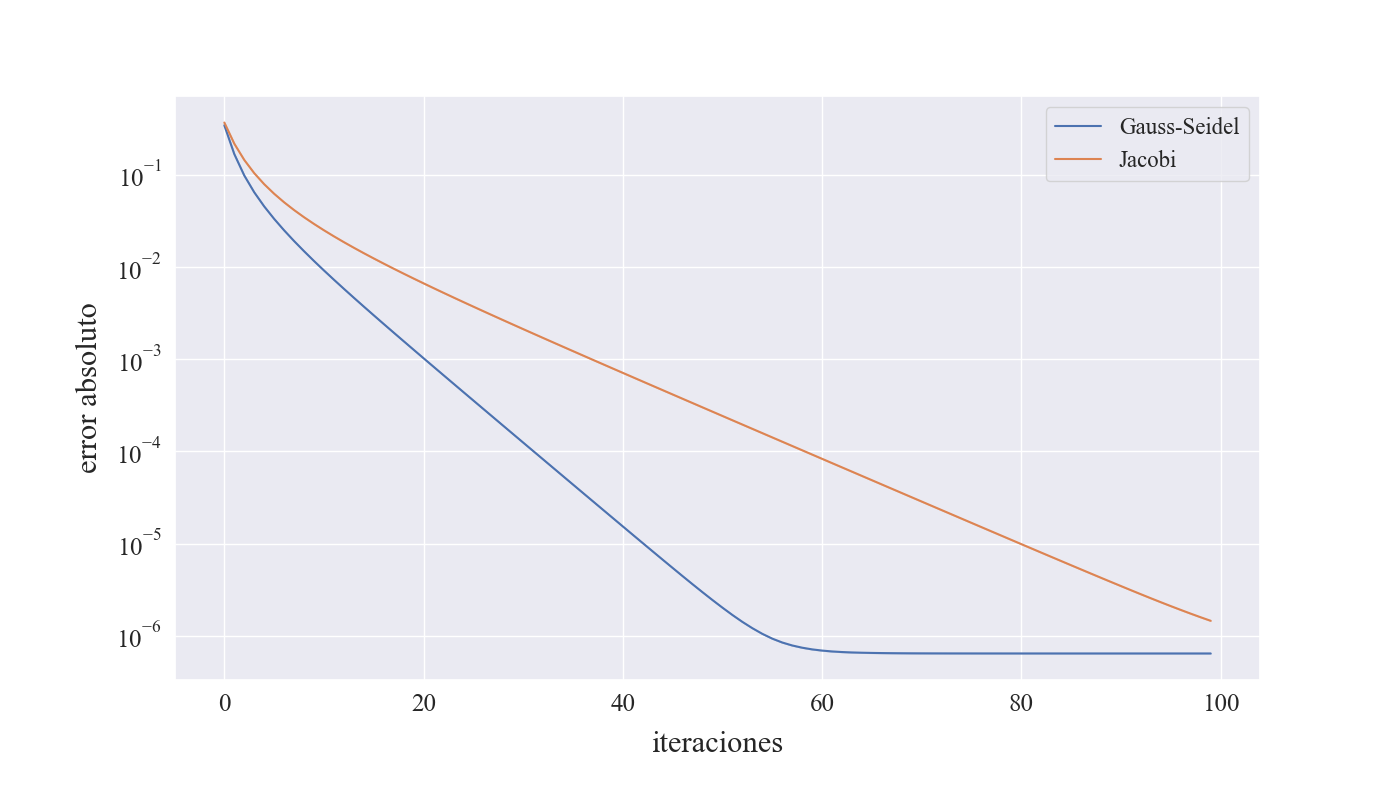
\includegraphics[width=1\textwidth, trim=0 0 0 30]{files/src/.media/convergencia_test_15_segundos.png}
    \caption{Error absoluto $L_1$ para el grafo del test \textit{15\_segundos}, con $n = 2000$ y $p = 0.9$, en función de la cantidad de iteraciones realizadas, para ambas implementaciones de \textit{PageRank} (escala logarítmica).} \label{test_15_segundos}
\end{figure}

%\vspace{1em}
\newpage
\begin{figure}[!htbp]
    %\ContinuedFloat
    \centering
    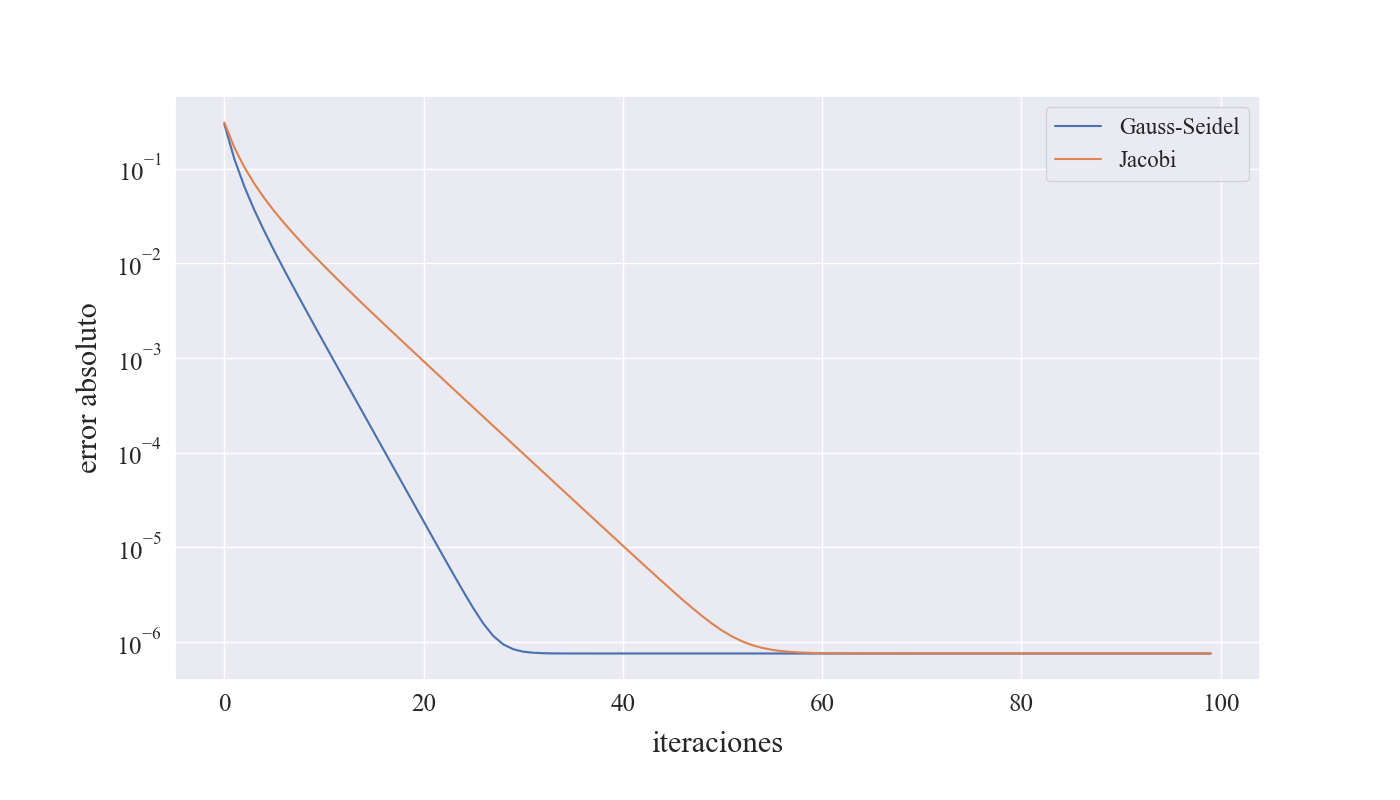
\includegraphics[width=1\textwidth, trim=0 0 0 10]{files/src/.media/convergencia_test_30_segundos.png}
    \caption{Error absoluto $L_1$ para el grafo del test \textit{30\_segundos}, con $n = 3000$ y $p = 0.8$, en función de la cantidad de iteraciones realizadas, para ambas implementaciones de \textit{PageRank} (escala logarítmica).} \label{test_30_segundos}
\end{figure}

%\vspace{1em}
\begin{figure}[!htbp]
    %\ContinuedFloat
    \centering
    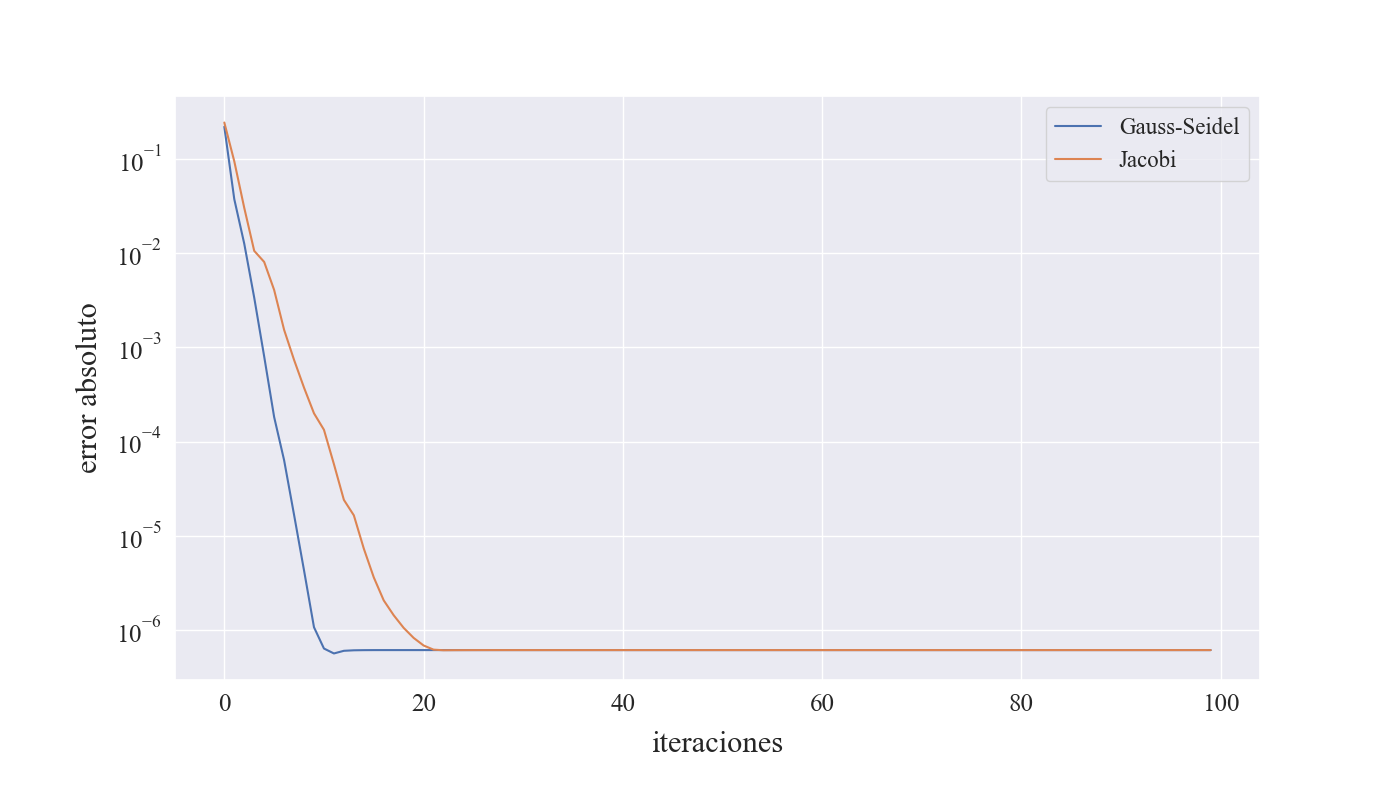
\includegraphics[width=1\textwidth, trim=0 0 0 30]{files/src/.media/convergencia_test_aleatorio_desordenado.png}
    \caption{Error absoluto $L_1$ para el grafo del test \textit{desordenado}, con $n = 5$ y $p = 0.76$, en función de la cantidad de iteraciones realizadas, para ambas implementaciones de \textit{PageRank} (escala logarítmica).} \label{test_aleatorio_desordenado}
\end{figure}

%\vspace{1em}
\begin{figure}[!htbp]
    %\ContinuedFloat
    \centering
    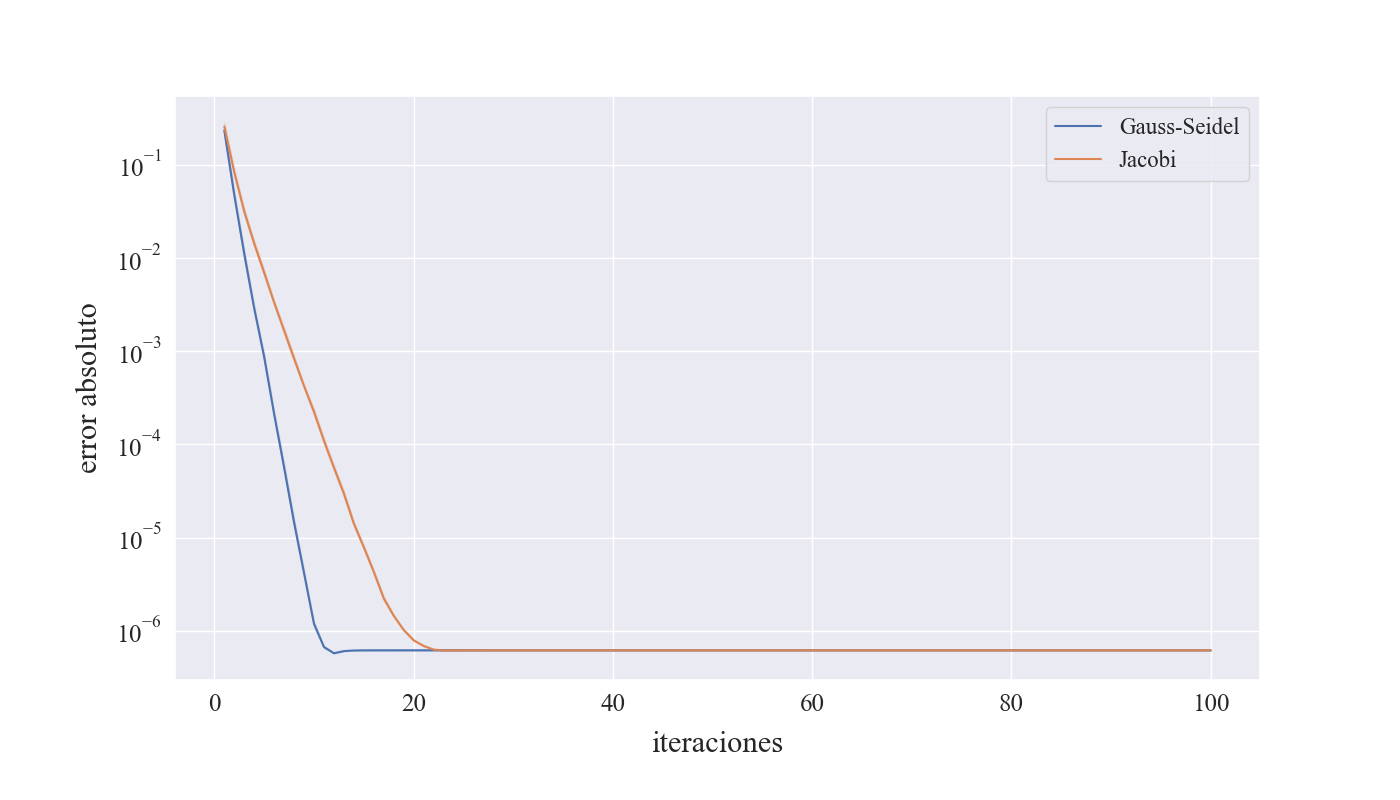
\includegraphics[width=1\textwidth]{files/src/.media/convergencia_test_aleatorio.png}
    \caption{Error absoluto $L_1$ para el grafo del test \textit{aleatorio}, con $n = 5$ y $p = 0.76$, en función de la cantidad de iteraciones realizadas, para ambas implementaciones de \textit{PageRank} (escala logarítmica).} \label{test_aleatorio}
\end{figure}

%\vspace{1em}
\begin{figure}[!htbp]
    %\ContinuedFloat
    \centering
    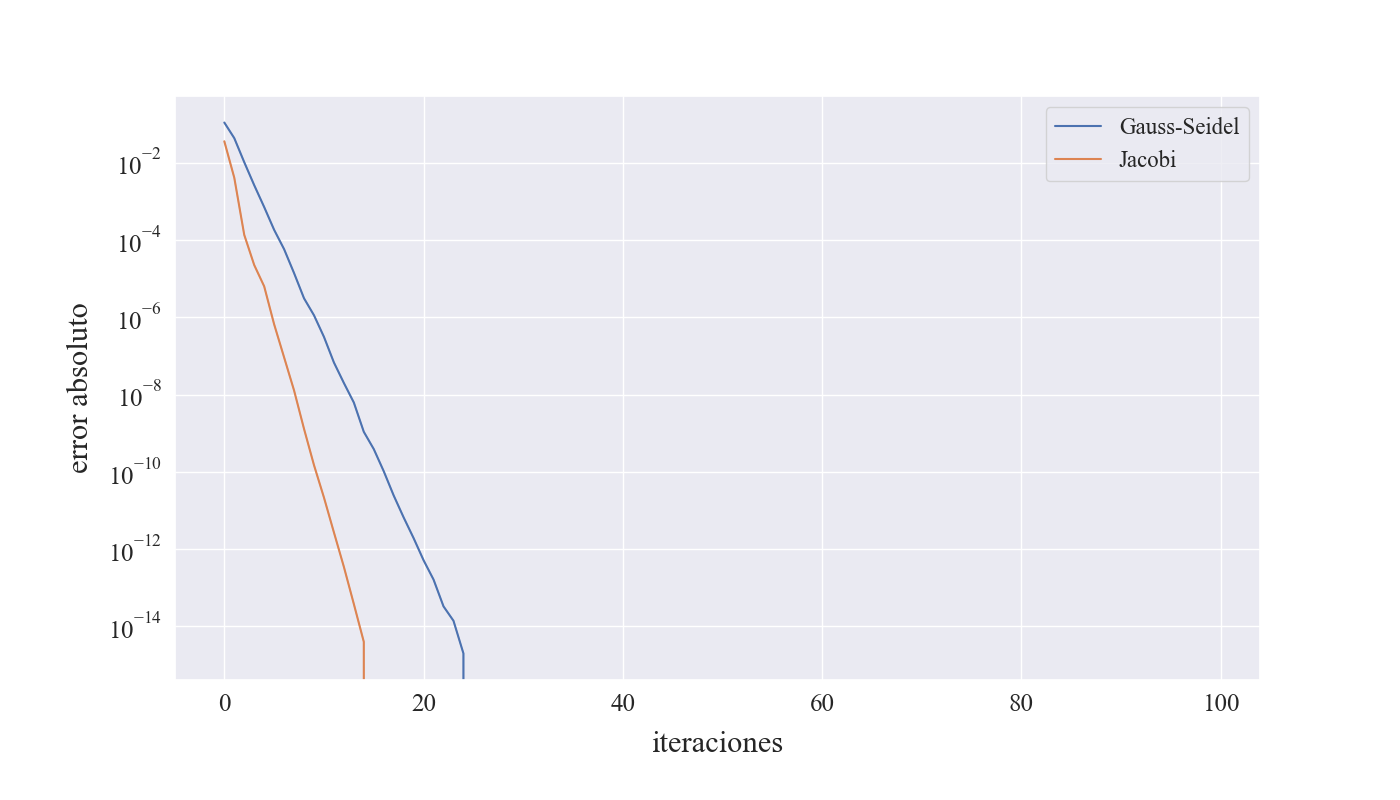
\includegraphics[width=1\textwidth]{files/src/.media/convergencia_test_completo.png}
    \caption{Error absoluto $L_1$ para el grafo del test \textit{completo}, con $n = 5$ y $p = 0.5$, en función de la cantidad de iteraciones realizadas, para ambas implementaciones de \textit{PageRank} (escala logarítmica).} \label{test_completo}
\end{figure}

%\vspace{1em}
\begin{figure}[!htbp]
    %\ContinuedFloat
    \centering
    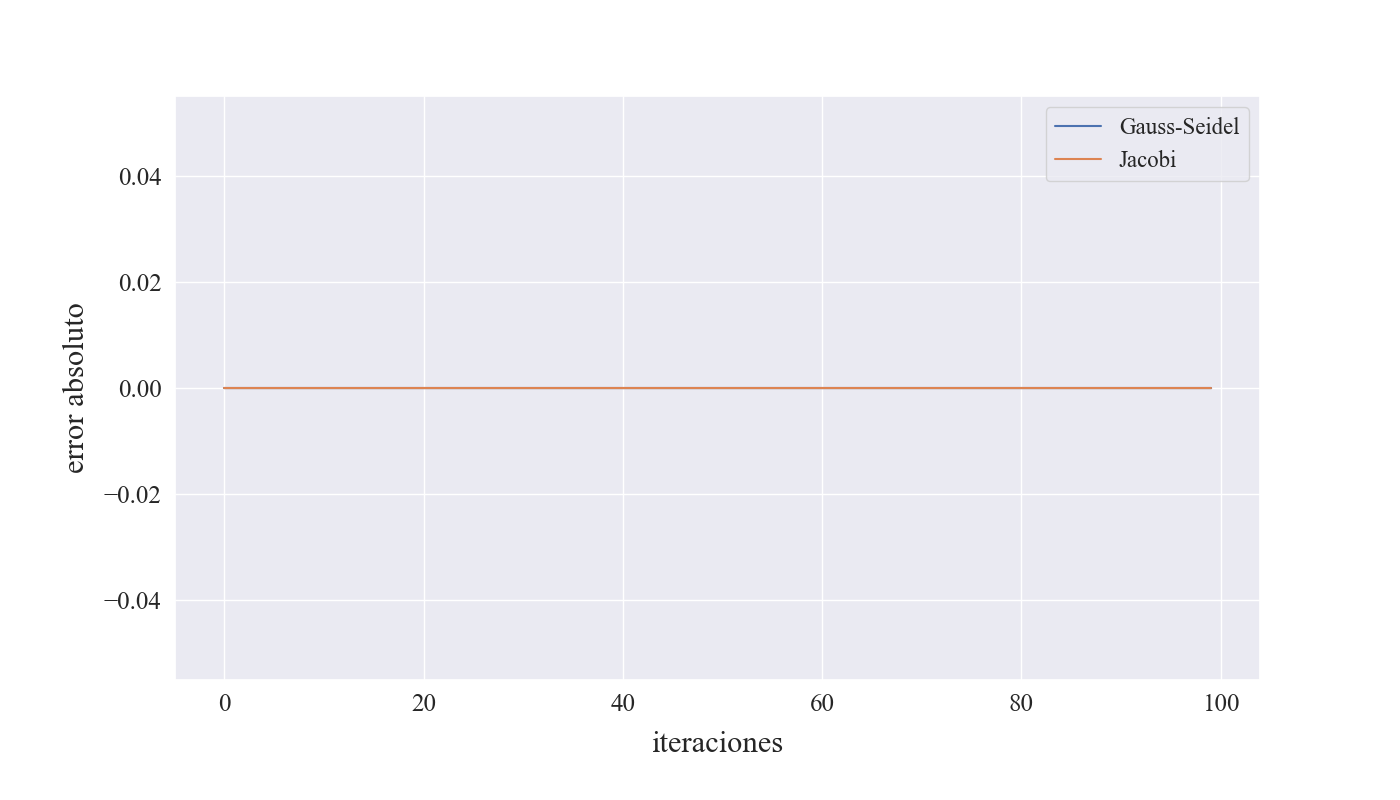
\includegraphics[width=1\textwidth]{files/src/.media/convergencia_test_sin_links.png}
    \caption{Error absoluto $L_1$ para el grafo del test \textit{sin\_links}, con $n = 5$ y $p = 0.64$, en función de la cantidad de iteraciones realizadas, para ambas implementaciones de \textit{PageRank}.} \label{test_sin_links}
\end{figure}

%\vspace{1em}
\begin{figure}[!htbp]
    %\ContinuedFloat
    \centering
    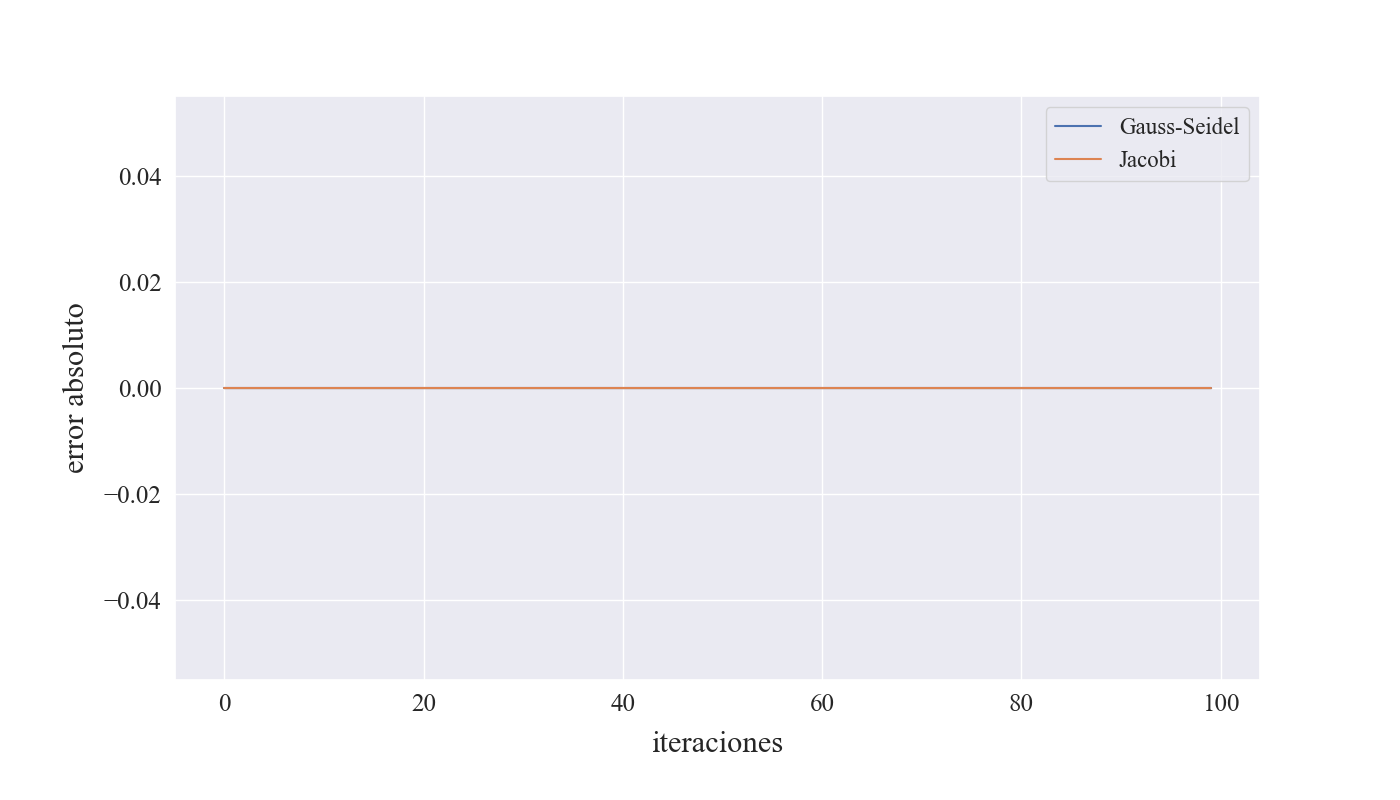
\includegraphics[width=1\textwidth]{files/src/.media/convergencia_test_trivial.png}
    \caption{Error absoluto $L_1$ para el grafo del test \textit{trivial}, con $n = 1$ y $p = 0.3$, en función de la cantidad de iteraciones realizadas, para ambas implementaciones de \textit{PageRank}.} \label{test_trivial}
\end{figure}

\vspace*{1em}
Procedemos a mostrar los resultados finales para el error absoluto con norma $L_1$ y $L_{\infty}$ ---para hacer una comparación por coordenadas---, tras las cien iteraciones:

\vspace{1em}
\begin{figure}[!htbp]
        \begin{tabular}{ |c|c|c|c|c|c|c| } 
        \hline
                                & \multicolumn{2}{c|}{Jacobi}    & \multicolumn{2}{c|}{Gauss-Seidel} \\
        \hline
        test                    & $L_1$             & $L_{\infty}$      & $L_1$     & $L_{\infty}$ \\
        \hline
        15\_segundos            & $1.45 \times 10^{-6}$  & $9.76 \times 10^{-9}$  & $6.4 \times 10^{-7}$  & $5 \times 10^{-9}$ \\
        30\_segundos            & $7.54 \times 10^{-7}$  & $5 \times 10^{-10}$  & $7.54 \times 10^{-7}$  & $5 \times 10^{-10}$ \\
        aleatorio\_desordenado   & $6.18 \times 10^{-6}$  & $2.52 \times 10^{-7}$  & $6.18 \times 10^{-7}$  & $2.52 \times 10^{-7}$ \\
        aleatorio               & $6.18 \times 10^{-6}$  & $2.52 \times 10^{-7}$  & $6.18 \times 10^{-7}$  & $2.52 \times 10^{-7}$ \\
        completo                & $0$  & $0$  & $0$  & $0$ \\
        sin\_links              & $0$  & $0$  & $0$  & $0$ \\
        trivial                 & $0$  & $0$  & $0$  & $0$ \\
        \hline                  
        \end{tabular}       
    \bigskip
    \caption{Error absoluto $L_1$ y $L_{\infty}$ de los casos de test para las implementaciones de $PageRank$ sobre los métodos de \textit{Jacobi} y \textit{Gauss-Seidel}.} \label{convergencia_resultados}
\end{figure}

\newpage

\section{Evaluación temporal}
\subsection{Casos de test}

Para comenzar el análisis sobre el tiempo de ejecución que demora cada uno de los métodos, decidimos inicialmente estudiar como se comportan estos frente a los test de la cátedra. A partir de los resultados logramos obtener mayor claridad sobre como se desenvolvían los métodos en distintos casos. Para luego poder generar con una intuición orientada los tests más profundos.

\vspace{2em}
\noindent\textsc{Metodología}. Inicialmente se definio un $epsilon = 10^{-6}$. Para cada uno de los test de la cátedra se realizó el cálculo de pagerank con el epsilon mencioniado para la eliminación gaussiana y se calculó $||x - res||_1$ donde $x$ refiere a la verdadera solución y $res$ al resultado que se obtuvo a partir de pagerank. Cabe destacar que este es un proceso determinístico. 

\vspace{2em}

Por otro lado, para el \textit{método de Jacobi} y para el \textit{método de Gauss-Seidel}, realizamos un binary-search donde en cada paso alteramos la tolerancia y calculamos el resultado. Editamos los límites de la tolerancia concorde el error calculado es mayor o menor que el error usando PageRank. Al finalizar este procedimiento obtuvimos tolerancias tales que, al calcular el error de comparar las respuestas que conceden \textit{Jacobi} y \textit{Gauss-Seidel} con la original, sea similar, en orden de magnitud, al error entre la respuesta que retorna PageRank y la original. De este modo podríamos realizar una comparación de tiempo de ejecución ``justa", donde todos los métodos obtengan una respuesta con un error muy similar.

\vspace{2em}

Luego para cada test, teniendo en cuenta las consideraciones previamente mencionadas, realizamos el cálculo 1 vez por método. Repetimos este paso 10 veces para atenuar las fluctuaciones de tiempo de ejecución que genera el computador y calculamos el promedio de cada método. Los resultados se pueden ver en la siguiente Figura. 

\vspace{2em}
*Inserte Gráfico de barras*
Como se puede apreciar en el gráfico, el \textit{método de Gauss-Seidel} y el \textit{método de Jacobi}, son considerablemente más rápidos cuando el tamaño de la matriz es grande a pesar de que el resultado obtenido es de la misma calidad para los tres métodos en todos los casos de test.

% DENSIDADES
\vspace{2em}
\subsection{En función de la densidad del grafo de entrada}

\newpage

% conclusiones
\section{Conclusiones}
A lo largo de este trabajo hemos evaluado distintos métodos para la resolución de sistemas lineales. Particularmente, nos concentramos en la aplicación de la \textit{eliminación gaussiana} y de los métodos de \textit{Gauss-Seidel} y \textit{Jacobi} en el contexto del algoritmo de \textit{PageRank}. 

Con el objetivo de medir sus velocidades de ejecución, planteamos una serie de experimentos que nos permitieron estudiar el comportamiento de las distintas implementaciones sobre una gran variedad de familias de grafos: redes aleatorias, de sumidero, completas, estrella y viborita. Esto lo realizamos en función de la densidad de las conexiones, sobre el total de los nodos, para cada entrada.

Además, medimos la velocidad de convergencia en función de la cantidad de iteraciones realizadas y la velocidad de ejecución de una serie de casos de test selectos.

\vspace{1em}
Observamos que los métodos iterativos son significativamente más rápidos que la eliminación gaussiana. A modos prácticos, operan en un orden de complejidad temporal menor, si bien la cantidad de iteraciones $q$ puede resultar significativa. Lo que es más, entre ambos métodos iterativos notamos que el método de \textit{Gauss-Seidel} se ejecutó ---en términos generales--- con mayor velocidad que el método de \textit{Jacobi}. Consideramos que esto se debe a que, dentro de una misma iteración, el primer algoritmo considera datos más recientes que el segundo.

\vspace{1em}
Si bien ambos métodos están restringidos en su aplicación ---la \textit{eliminación gaussiana} funciona solo para matrices con factorización \textit{LU} y los métodos iterativos sólo sobre el conjunto de matrices para los que convergen---, de tener la posibilidad de elección, los algoritmos de \textit{Gauss-Seidel} y \textit{Jacobi} prueban ser más eficientes a la hora de resolver sistemas lineales.
\newpage

% apendice
\section{Apéndice}
\input{files/src/apendice.tex}

%\newpage
% bibliografia - requiere que haya citas
%\bibliographystyle{plain}
%\bibliography{files/citations.bib}
%\newpage

\end{document}
